\subsection{Definitions}
We here define a food web as the directed network representing all energy fluxes in an ecosystem. Vertices and edges represent species (either consumers or resources) and their interactions, respectively. 
An example (Fig. \ref{FIG:web}) highlights the basic nutrient source, typically sunlight or sugar, primary producers (autotrophs), such as plants, their consumers, and omnivores.  
We here measure a species' trophic level, $l$, as the weighted mean of its resources' levels incremented by one.
Primary producers are distinct in that at they only consume basic nutrient sources, i.e. they always have $l = 1$.

\subsection{Model}
We here focus exclusively on consumer-resource interactions, and do not consider mutualism \cite{bastolla2009architecture}, parasitism \cite{combes2001parasitism}, or the detritus network \cite{moore2004detritus}, that is, energy stored in deceased biomass.
We further restrict to a single basic nutrient source, and require that species feeding on basic nutrients are never omnivorous \cite{agrawal2000omnivores}, e.g. that plants do not consume other plants.

\begin{figure}
	\centering
		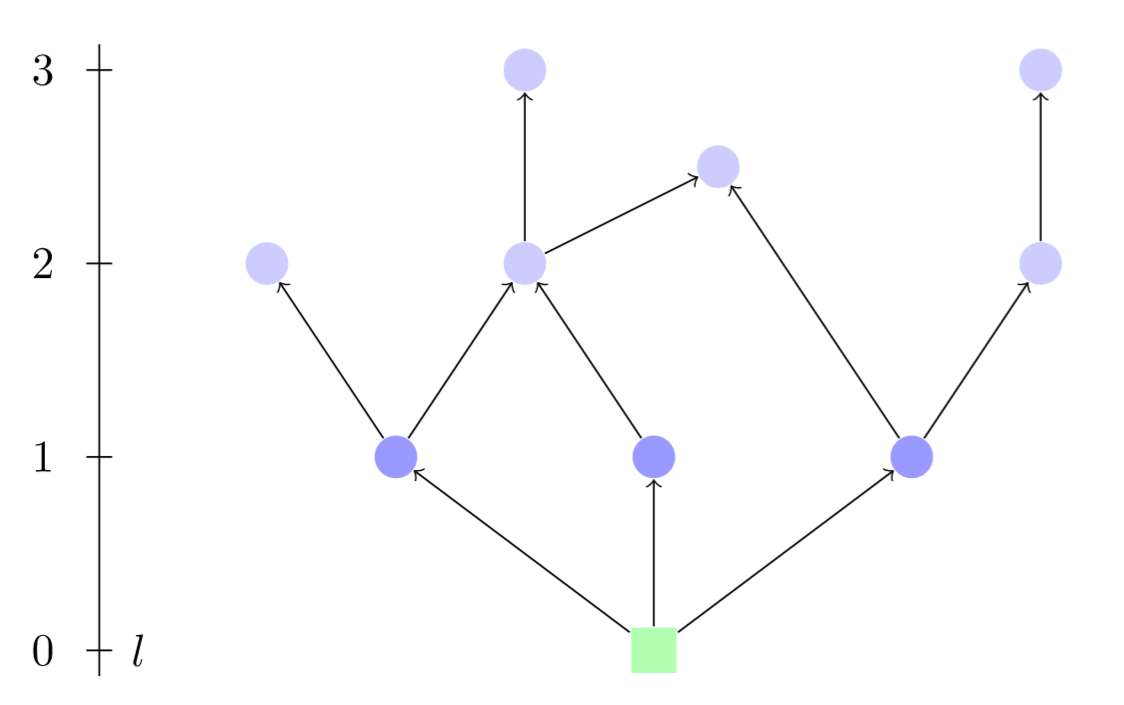
\includegraphics[scale=.55]{figs/web.png}
	    \caption{\textbf{Example of a food web.} The green square is the basic nutrient source. The dark and light blue circles are the primary producers and the species consuming other species (including primary producers), respectively. The black lines represent consumer-resource interactions where the arrows point in the direction of the energy flux. 
        The axis on the left illustrates the trophic levels, $l$.}
	    \label{FIG:web}
\end{figure}

The Lotka-Volterra equations \cite{lotka1926elements,volterra1927variazioni} describe spatially and temporally homogeneous, %well-mixed, 
consumer-resource relations. A generalization of these \cite{hofbauertheory, campbell1961conditions, drossel2003handbook} can be used to describe the dynamics of larger, more complex food webs. 
For primary producers the generalized Lotka-Volterra equations are
\begin{equation}
        \frac{\dot{S_i}}{S_i} = k_i \left( 1 - \sum_j^{n_1} S_j \right) - \alpha_i - \sum_k^{n} \eta_{ki} S_k, \label{eq:LV_i}\; \\
\end{equation}
where $n_1$ denotes the total number of primary producers and $S_i$, $i\in\{1,\dots,n_1\}$, denotes the population density of a species in units of biomass, normalized to its carrying capacity. 
It is thereby assumed that all primary producers exclusively consume the same basic nutrient source. 
For all other species, $S_k$, $k\in\{n_1+1,\dots,n\}$ with $n$ the total number of species in the food web, the equations read 
\begin{equation}
     \frac{\dot{S_k}}{S_k} =  \sum_{m=1}^{n} \beta_{km}\eta_{km} S_m - \alpha_k - \sum_{p=n_1+1}^{n} \eta_{pk} S_p\;. \label{eq:LV_k}
\end{equation}

Here $S_k$ is again measured in units of normalized biomass. 
Eqs. (\ref{eq:LV_i}) and (\ref{eq:LV_k}) capture the relative change in population density in time, for primary producers and all remaining species, respectively. 
In Eq. (\ref{eq:LV_i}), $k_i>0$ denotes the growth rate of the primary producer $S_i$, that is the maximal reproduction rate at unlimited nutrient availability.
The sum on $S_j$'s represents logistic growth, representing nutrient depletion by all primary producers. 
In Eqs (\ref{eq:LV_i}) and (\ref{eq:LV_k}), $\alpha_j>0$ is the decay rate of a species $S_j$, representing death not caused by consumption through other species. 
$\eta_{ki}\geq 0$ is the link-specific interaction strength between consumer $S_k$ and resource $S_i$. 
On the RHS of either equation, note the final term representing the diminishing effects experienced by resource species --- caused by consumption. 
This term is mirrored by the first term in Eq.~(\ref{eq:LV_k}), which describes the strengthening effect on the consumer side.
The coefficients $\beta_{ki}\leq 1$ encode link-specific consumption efficiency --- that is, potentially incomplete use of energy removed from a resource species by its consumer.

The equations describe a simplified food web where consumption is modeled by the simple type-I response \cite{holling1959components}, where consumer resource fluxes scale proportional to the product of consumer and resource density, without saturation effects.
Moreover, Eqs (\ref{eq:LV_i}) and (\ref{eq:LV_k}) describe a rigid food web in that the species are incapable of adapting their consumption behavior to changes within the food web, such as a decreasing population of resources or competition from an invasive species \cite{beals1999predator}. 


%\subsection{Feasibility}
%A food web is feasible if the fixed points of the Lotka-Volterra equations are positive, that is if all species have positive steady states. Exploiting the linearity of Eqs. (\ref{eq:LV_i}) and (\ref{eq:LV_k}), feasibility can be examined by setting the left hand side (LHS) to zero and rearranging
%\cite{haerter2016food}, yielding
%\begin{align}
%    \frac{k_i - \alpha_i}{k_i} &= \sum_j^{n_1} S_j + \sum_k^{n} \frac{\eta_{ki}}{k_i} S_k,  \label{eq:R_i} \\
%    \alpha_k &= \sum_i^{n} \beta_{ki}\eta_{ki} S_i - \sum_p^{n} \eta_{pk} S_p\;, \label{eq:R_k}
%\end{align}
%which is equivalent the matrix equation $\mathbf{K} = \mathbf{R}\cdot \mathbf{S^*}$. 
%Here $\mathbf{K}$ are the constants on LHS, collected in a vector. $\mathbf{R}$ is the interaction matrix, i.e. a matrix containing the interaction parameters. 
%The fixed points are collected in a density vector, $\mathbf{S^*}$. 
%This yields the following equation for the steady states:
%\begin{equation}
%    \mathbf{S^*} = \mathbf{R}^{-1}\cdot \mathbf{K}, \label{eq:S*} 
%\end{equation}
%and it follows that food webs with invertible interaction matrices have unique steady states. 
%Feasibility then requires, that all $\mathbf{S^*}$ be positive.
%For tree-like food webs, it was shown that parameters could be chosen, to ensure feasibility, once inversion of $\mathbf{R}$ was possible \cite{haerter2016food}.
%For more general food webs, as the ones explored here, the test for feasibility must generally be performed numerically.


\subsection{Feasibility and Stability}
A food web is feasible if the fixed points of the Lotka-Volterra equations are positive, that is if all species have positive steady states. Using some basic algebraic operations on eqs. (\ref{eq:LV_i}) and (\ref{eq:LV_k}), these simplify to the matrix equation $\mathbf{K} = \mathbf{R}\cdot \mathbf{S^*}$ \cite{haerter2016food}. %supplementary?
Here $\mathbf{K}$ are the constants on LHS, collected in a vector. $\mathbf{R}$ is the interaction matrix, i.e. a matrix containing the interaction parameters. 
The fixed points are collected in a density vector, $\mathbf{S^*}$. 
This yields the following equation for the steady states:
\begin{equation}
    \mathbf{S^*} = \mathbf{R}^{-1}\cdot \mathbf{K}, \label{eq:S*} 
\end{equation}
and it follows that food webs with invertible interaction matrices have unique steady states. 
Feasibility then requires, that all $\mathbf{S^*}$ be positive.

Feasibility of a food web does not ensure its sustainability as the steady states might represent unstable fixed points.
%Only if the steady state is globally stable, will the populations with certainty return this equilibrium. 
%For real food webs, which consist of discrete organisms, even a globally stable food web might not be sustainable, as the disturbance might induce oscillations to unphysically small densities. 
%Furthermore, stability does not hedge against invasions. Adding an invader species to an existing food web yields a new set of Lotka-Volterra equations that might represent an unstable or even unfeasible system.
For small perturbations away from equilibrium, linear stability of the steady states can be determined from the eigenvalues of the community matrix, $\mathbf{C}$, that is the Jacobian of the Lotka-Volterra equations evaluated at the fixed points
\begin{equation}
    \mathbf{C} = \mathbf{J}_{\mathbf{S^*}} = \sum_i^n\sum_j^n \frac{\partial \dot{S_i}(\mathbf{S^*})}{\partial S_j}.
    \label{eq:C}
    %\nonumber
\end{equation}
Here $\dot{S_i}$ and $S_j$ are the time derivatives and densities of eq. (\ref{eq:LV_i}) and (\ref{eq:LV_k}), and $\mathbf{S^*}$ is the steady states from eq. (\ref{eq:S*}).
%The real part of an eigenvalue determines the direction of the change in a density when it is locally displaced from its steady state. Negative real parts correspond to attraction towards the steady state, whereas positive real parts correspond to repulsion \cite{nemytskii2015qualitative}. The imaginary parts determine whether or not the density is also oscillating as it approaches or reproaches the steady state.
The food web is linearly stable if all eigenvalues of the community matrix have negative real parts. This corresponds to local attraction towards the steady states \cite{strogatz2018nonlinear}.

The eigenvalue spectrum of a random matrix is shown to approach a circle as the size of the matrix increases \cite{tao2010random}. Based on this, it has been argued that large and complex food webs are almost certain to be unstable \cite{may1972will}.

However, real food webs are believed to have non-random interaction patterns and might not be accurately modelled as a random matrix \cite{sih1990interacting, allesina2012stability}.
Real ecosystems are not a random collection of species and interactions, but a network that has evolved non-randomly for billions of years \cite{weiss1998evolution}, hence it is uncertain how accurate these stability criteria are for food webs.

